\chapter{About the technology stack}
\label{cha:techstack}

Before describing the entire project, we need to know what we are talking about. In particular, there are the software and libraries strongly used in the project:  
\begin{itemize}
    \item ROS2
    \item Gazebo
    \item \acrfull{rviz}
    \item \acrfull{nav2}
    \item Docker
\end{itemize}

\section{\acrshort{ros}2}

\begin{wrapfigure}{l}{0.2\textwidth}
    
\includegraphics[width=0.2\textwidth]{images/foxy}
\end{wrapfigure}

\textit{\acrshort{ros}2, which stands for Robot Operative System 2, is a set of software libraries and tools for building robot applications.}\cite{ros2desc} On it, every process is a node and each node has the possibility to talk to other ones thanks to some channel of communications called topics using the publish/subscribe model.

This version of \acrshort{ros}2, called \textbf{Foxy Fitzroy}, was used because it is possible to integrate the \textit{plansys2} libraries used for planning.

Thanks to \Acrshort{ros} \textit{hardware abstraction, low-level device control, implementation of commonly-used functionality, message-passing between processes, and package management}\cite{ros2help}, the developer can ignore specific hardware details and software implementations and focus only on the application itself. 

This means that executing a \acrshort{ros} node on your own computer is the same of executing it on a robot, as long as you are using the same operative system (only \textbf{Ubuntu 20.04}) and the same external devices, if you are not simulating them.

\section{Gazebo}
\label{sec:gazebo}

\begin{wrapfigure}{r}{0.25\textwidth}
    
\includegraphics[width=0.25\textwidth]{images/gazebo}
\end{wrapfigure}

Gazebo is a simulation suite. It lets you create and simulate things with the bundled physic and render engines, alongside a variety of sensors.

It comes as a standalone software, but thanks to its interfaces it is possible to integrate it with \acrshort{ros}2, using several packages developed for this purpose: in this way you can simulate both robots and the environments in which they operate, before actually moving to the real world, or test your last modifications even if you are somewhere other than the real robot location.

With the sensors and the plugins you are able to simulate lasers (e.g. lidars), cameras (e.g. depth cameras), IMUs and GPS receivers, or also differential drive and joints state.

\section{\acrfull{rviz}}

\begin{wrapfigure}[7]{l}{0.25\textwidth}
    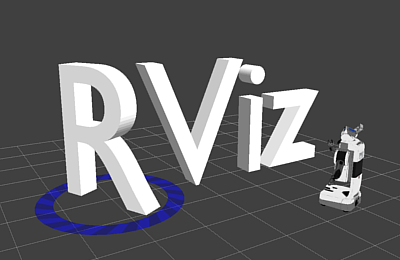
\includegraphics[width=0.25\textwidth]{images/rviz}
\end{wrapfigure}

\Acrshort{rviz}, is a visualization tool for ROS: you can visualize the sensors, the robots, the environment, and also the algorithms; in general, you can see the actual state of your \acrshort{ros} system. In this project it has been used to set initial robot position on the map, see room boundaries, obstacles and visualize the path the robot is currently following to reach the goal, that could be specified graphically (manually) or by some other nodes (automatically). 

\section{\acrfull{nav2}}

The Navigation Stack is a collection of packages of \acrshort{ros}2 providing useful tools for the navigation of your robot: path planning, localization, obstacle avoidance, recovery from collisions, mapping and so on\footnote{A detailed description can be found in \autoref{cha:navigation}}. These packages were used as a basis for this project: in such a manner you do not have to worry about the navigation algorithms, you just need to pass sensor information, and they will do the rest; moreover, you can use the provided interfaces to customize and automate the whole process of navigation.

It can be thought as a template for navigation systems with a generic configuration, but thanks to \Acrshort{ros}, you can set what parameters you want for each node easily with a YAML file: this will be parsed when you launch the navigation stack and the nodes will be configured accordingly.

\begin{figure}[h]
    % \noindent\makebox[0.9\textwidth]{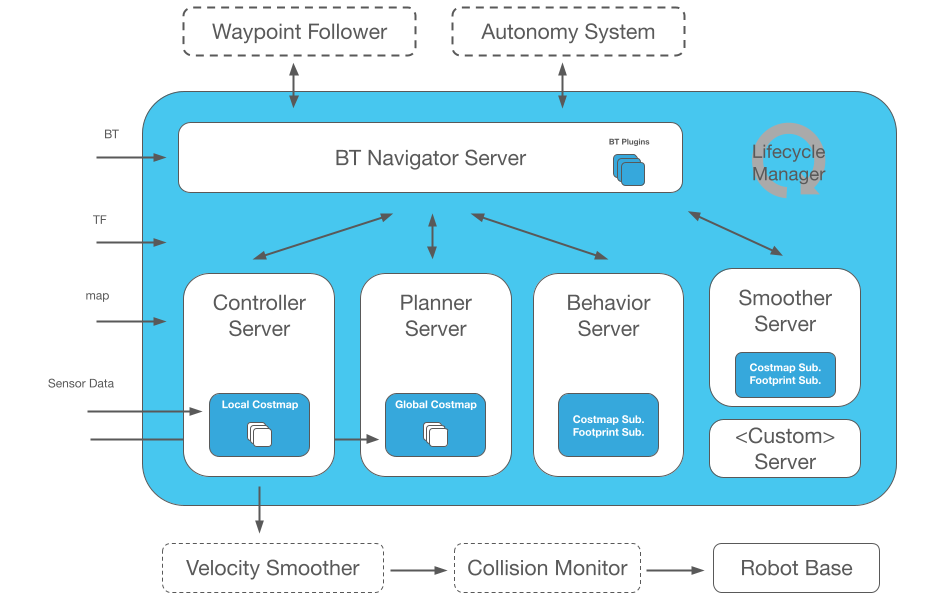
\includegraphics[width=0.9\paperwidth]{images/nav2_architecture}}
    \centering
    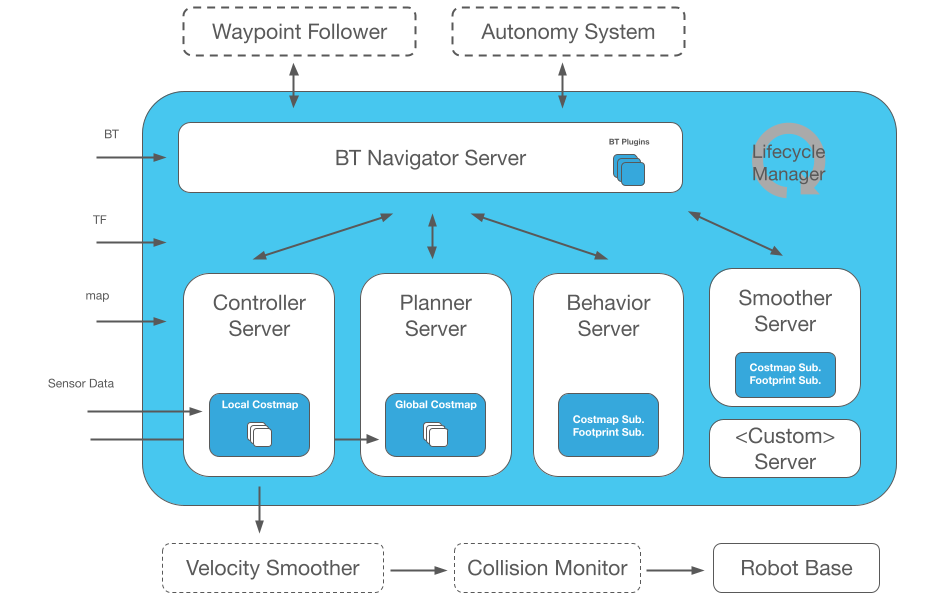
\includegraphics[width=0.8\textwidth]{images/nav2_architecture}
    \caption{Navigation architecture}
\end{figure}

\section{Docker}
  
\begin{wrapfigure}[3]{r}{0.15\textwidth}
    
\includegraphics[width=0.15\textwidth]{images/docker}
\end{wrapfigure}
  
Docker is a platform that let you separate your application using an isolated environment called container. It gives you also the possibility to run multiple containers at the same time. As it was originally designed, Docker was used in this project for the following reasons: % basta? (?)
  
\begin{itemize}
    \item \textbf{separate} this project workspace from all the other ones, to \textbf{avoid conflicts}
    \item keep the workspace \textbf{equal} for \textbf{every device} (real robot or simply a computer)
    \item permit development on any device \textbf{not running} necessarily \textbf{Ubuntu 20.04} (required from \acrshort{ros}2) as its OS
\end{itemize}  
  
Inside a Dockerfile, a file containing instructions on how to build an image\footnote{It is used as a starting point when launching a container} with your own configurations, were typed all the commands required to install the missing packages from the base image already containing basic \acrshort{ros}1 and \acrshort{ros}2 packages \cite{dockerimage}. The complete Docker setup can be found in \autoref{cha:dockerfile}.